\chapter{\IfLanguageName{dutch}{Stand van zaken}{State of the art}}
\label{ch:stand-van-zaken}

Zoals eerder vermeld focust dit onderzoek zich op Security Information and Event Management en wat de eigenschappen en uitdagingen zijn gerelateerd aan het gebruik hiervan.
Om een netwerkinfrastructuur goed te beveiligen, is het belangrijk dat men de omgeving begrijpt en weet welke componenten dit opbouwen. Daarom werd er eerst gekeken naar verschillende log types en op welke manier een SIEM in elkaar zit en werkt.
Daarna ging de aandacht naar de selectiecriteria en wat aan welke zaken er moet gedacht worden alvorens de implementatie.
Als laatste werd er gekeken naar een aantal SIEM producten op de markt. Over deze tools werd een korte beschrijven gegeven gaande van hun functionaliteiten tot hun sterktes en zwaktes. Voor dit werd gebruik gemaakt van Het Gartner Magic Quadrant. 
\section{\IfLanguageName{dutch}{Geschiedenis}{Problem Statement}}

De term Security Information and Event Management, bedacht door Mark Nicolett en Amrit Williams in 2005, beschrijft de mogelijkheden om informatie te verzamelen, analyseren en presenteren [Eva Kostrecova]. SIEM is een combinatie van Security Information Mangement (SIM) en Security Event Management (SEM) functionaliteiten in één security management systeem. 
SIM focust vooral op het verzamelen en analyseren van historische data bedoelt voor het verbeteren van opslag prestatie in IT infrastructuur. Daartegenover staande is SEM, dat voornaamlijke focust op aggregatie van data en deze voorstelt in een overzichtelijk formaat dat helpt bij het afhandelen van security incidenten. \autocite{Morteza Zeinali} Sommige onderzoekers spreken liever van 'SIEOM' en voegen sinds kort de O voor 'opportunity' toe. Dit is omdat rapporten en waarschuwingen van een SIEM-omgeving de mogelijkheid bieden, de veiligheid van systemen te verbeteren \autocite{Dorigo2012}.

\section{\IfLanguageName{dutch}{Wat is SIEM}{Problem Statement}}

SIEM bestaat uit een groot aantal producten en services voor het gelijktijdig beheren van beveilingingsinformatie en gebeurtenissen. SIEM staat ook in voor analyse van beveilingsrisico's en incidenten op regelmatige basis. SIEM is dus nuttig voor het detecteren van bedreigingen, het onderzoeken van problemen die verband houden met eerdere beveilingsrisico's, het uivoeren van een onmiddelijke respons op incidenten en het voorbereiden van rappporten om de gebruiker zo goed mogelijk te informeren. Dit alles maakt het makkelijker om bepaalde trends en patronen op te merken die misschien niet altijd vanzelfsprekend zijn. De laatste jaren zijn er steeds meer IT implementaties en worden mensen steeds meer afhankelijker van technologie. Het pijnlijk gevolg is dat er een grote stijging in het aantal aanvallen en dit heeft er voor gezorgd dat steeds meer bedrijven en organisaties het nut inzien van IT-beveiliging en hun netwerkmonitoring te verbeteren.

\subsection{\IfLanguageName{dutch}{Security Operations Center}{Problem Statement}}

Een SIEM biedt een goede technische basis voor een Security Operations Center (SOC) door gebruik te maken van vele processen die samenwerken om zo snel mogelijk op beveiligingsincidenten te reageren.

Een SOC vertegenwoordigt het organisatorisch aspect van een beveiligingsstrategie in een onderneming door het samenbrengen van processen, technologieën en mensen. Het bestaat niet uit één enkele entiteit maar uit een complexe structuur om de algehele beveiliging van een organisatie te verbeteren. Een SOC integreert, controleert en analyseert verschillende beveiligingsrelevante systemen en gebeurtenissen in één organisatorische eenheid. Om de technische kant van de beveilingsoperaties, dat een SOC gewoonlijk gebruikt, te realiseren, wordt er onder andere gebruik gemaakt van SIEM-systemen \autocite{Vielberth2021}. 

\subsection*{\IfLanguageName{dutch}{SOC functies}{Problem Statement}}

FIGUUR VAN SOC ARCHITECTUUR

De figuur toont een algmeen framework van de verschillende functies en componenten dan men typisch terugvindt in een SOC \autocite{Schinagl; Paas: Schoon, 2015}.

\begin{itemize}
    \item \textbf{Intelligence function}
    
    Dit is de kern van een SOC en kan vergeleken worden met een Computer Emergency Response Team (CERT). Dit team bestaat veelal uit analysten dat informatie uitwisselen met interne en externe partijen over potentiële beveiligingsincidenten.
    
    \item \textbf{Baseline Security function}
    
    Dit is de component dat toezicht houdt de operationele processen voor het beter beveiligen van servers, besturingssystemen en netwerkapparaten, en voert kwetsbaarheids- en compliancescans uit. Compliancescans houdt in dat er wordt onderzocht of het systeem voldoet richtlijnen dat binnen een organisatie of bedrijf moeten worden voldaan zoals Health Insurance Portability and Accountability Act (HIPAA) en Health Information Trust Alliance (HITRUST)
    
    \item \textbf{Monitoring function}
    
    observeert het dataverkeer en probeert afwijkingen te identificeren. Om dit te kunnen volbrengen, worden grote hoeveelheid loggegevens en signalen opgeslagen en gefilterd met behulp van dynamische regelsets. één van de uitdagingen bestaat erin om de SIEM zo af te stellen, dat alleen relevante alerts of events worden geïdentificeerd.
    
    \item \textbf{Penetration Test function  }  
    
    Penetratietests worden gebruikt om te bepalen hoe een systeem reagert op een aanval en of de verdediging van het systeem al dan niet kan worden doorbroken.
    
    \item \textbf{Forensic function}
    SOC-analysten staan in voor het vinden van details in dataverkeer en logs afkomstig van de infrastrcutuur.
    
    
    
\end{itemize}














\subsection{\IfLanguageName{dutch}{Architectuur}{Problem Statement}}

FIGUUR VAN SIEM ARCHITECTUUR

Figuur idk toont een veelvoorkomende architectuur van een SIEM, Als er dieper wordt ingegaan op de verschillende componenten: 

hellemaal onderaan staan de verschillende platformen en apparaten dat data beschikbaar stellen. Deze data wordt verazamelt door collectors, en dit kan via verschillende configuraties. typisch wordt een agent geïnstalleerd op het apparaat dat moet worden gemonitort, maar dit kan ook via een 'agentless' oplossing.
Een agent is een software dat het mogelijk maakt om data van verschillende apparaten in het netwerk te 




\section{\IfLanguageName{dutch}{SIEM implementatie}{Problem Statement}}

De huidige SIEM aanbieders zouden veel meer moeten aanbieden dan het beheren van logs. De beste aanbieders leveren geavanceerde statistische analyse, machine learning, en threat management tegen de nieuwste malware, adware en cyberaanvallen. SIEM-leveranciers moeten ervoor zorgen dat hun gebruikers de capaciteit hebben om beveiligingsgebeurtenissen en -risico's op de meest effectieve en efficiënte manier aan te pakken.  

\section{\IfLanguageName{dutch}{Providers}{Problem Statement}}

Deze sectie geeft een overzicht van de verschillende aanbieders dat beschikbaar zijn in de SIEM wereld. er wordt een ondersheid gemaakt tussen de aanbieders aan de hand van het magic quadrant, opgesteld door Gartner. Gartner is een onderzoeks- en adviesbureau op het gebied van informatietechnologie. De twee belangrijkste datavisualisatie- en analysetools van het bedrijf zijn Gartner Magic Quadrants en de hype-cyclus.

het Magic Quadrants is een onderzoeksmethodologie en visualisatie voor het monitoren en evalueren van de voortgang en postie van bedrijven en producten in een specifieke, op technologie gebasseerde markt. Magic Quadrants gebruikt een tweedimensionale martix om de sterke punten en verschillen tussen producten te illustreren. deze rapporten helpen lezers het product te vinden, die aan hun behoeften voldoen \autocite{Miller2019}.

de matrix is onderverdeeld in verschillende categorieën:

\begin{itemize}
    \item Leaders: deze bedrijven scoren goed op beide criteria. zowel het vermogen om uit te voeren als de volledigheid van hun visie zijn aanwezig. Dit zijn meestal de grotere, volwassen bedrijven die al langer op de markt zijn.
    
    \item Visionairen: begrijpen waar de markt naartoe gaat of hebben een visie voor veranderende marktregels, maar voeren nog niet goed uit. Dit zijn typisch de kleinere bedrijven.
    
    \item Niche spelers: concenteren zich met succes op een klein segment, of zijn ongericht en overtreffen niet en presteren niet beter dan anderen. Dit zijn meestal de nieuwe toevoegingen aan het Magic Quadrant.
    
    \item Challengers: presteren vandaag goed of kunnen een groot segment domineren, maar scoren lager op de volledigheid van hun visie.
\end{itemize}

In het Magic Quadrant worden verschillende aanbieders opgenomen, maar deze worden alleen toegevoegd als ze voldoen aan de marktdefinitie en inclusieciteria opgesteld door analysten bij Gartner.
Om een kort overzicht te geven, werden een aantal aanbieders bekeken die al enkele jaren sterk in de markt staan en die het meest interessant leken.

FOTO VAN MAGIC QUADRANT
\begin{figure}
    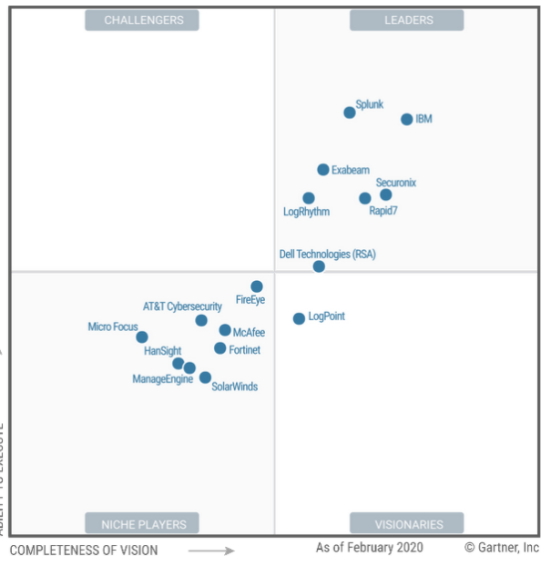
\includegraphics[scale=1.50]{gartner} haha
\end{figure}

\subsection{\IfLanguageName{dutch}{IBM QRadar}{Problem Statement}}

IBM QRadar staat al jaren op de leiderspositie in het Magic Quadrant van Gartner. Het is een tool dat geschikt is voor 
zowel kleine als grotere implementaties. Qradar kan als een applicatie, een SaaS of een IaaS worden uitgevoerd.Componenten kunnen in een all-in-one oplossing gebruikt worden of apart geschaald met verschillende applicaties voor diverse functies. Er zijn ook hybride oplossingen mogelijk met lokaal QRadar,
SaaS gehost op de IBM Cloud en optioneel nog monitoring van op afstand.
QRadar bestaat uit volgende onderdelen:

\begin{itemize}
    \item QRadar Console: dit onderdeel biedt de interface aan met realtime gebeurtenissen en overtredingen, rapporten en administratieve beheerfuncties.
    
    \item Event Collector: verzamelt events van lokale en externe logs en normaliseeert deze gegevens, zodat ze door QRadar kunnen worden gebruikt.
    
    \item Event Processor: verzamelt events door gebruik te maken van een Custom Rules Engine (CRE). als events matchen met voorafgedefineerde regels uit de CRE, wordt een bepaalde actie uitgevoerd.
    
    \item QFlow Collector: Analyse van netwerkgedrag en detectie van anomalieën op het netwerk.
    
    \item vFlow Collector: Is ontworpen om virtualisatie te ondersteunen. Het heeft dezelfde functionaliteiten als QFlow
    
\end{itemize}

\textbf{Sterktes}

\begin{itemize}
    \item Snelle verzameling en verwerking van events.
    \item Makkelijk uitbreidbaar.
    \item Geschikt voor klein tot grote bedrijven.
    \item Eenvoudige installatie.
    
\end{itemize}

\textbf{Zwaktes}

\begin{itemize}
    \item Moet beheerd worden door ervaren gebruikers.
    \item Beperkte mogelijkheid om als gebruiker aanpassingen te doen.
    \item Complexe licentie opties. 
\end{itemize}


\subsection{\IfLanguageName{dutch}{Splunk}{Problem Statement}}

Splunk is een softwareplatform voor het analyseren en visualiseren van gegeneerde gegevens en logs die zijn verzameld via verschillende bronnen, zoals: websites, applicaties en apparaten waaruit een IT-omgeving is opgebouwt \autocite{Vardhan2020}.
Splunk zorgt ervoor dat gegevens en events in real-time beschikbaar zijn en worden samengebracht in een makkelijk bruikbaar, overzichtelijk dashboard. Op deze manier kunnen bedreigingen op een efficiënte manier worden aangepakt.
Splunk kan worden geïmplementeerd on-premises of via een cloud omgeving, waar de hosting, onderhoud en updates worden uitgevoerd door Splunk zelf. Een cloud implementatie brengt heel wat voordelen met zich mee, maar er moet altijd rekening gehouden worden met informatieveiligheid en hoe data wordt opgeslagen. In de volgende sectie wordt hier verder op ingegaan.

De belangrijkste componenten in de Splunk-architectuur zijn: Forwarder, Indexer en Search Head.

\begin{itemize}
    \item Forwarder: Dit is een agent (soort applicatie) dat geïmplementeerd wordt op IT-systemen, dat logs en data verzamelt van wat er gebeurt op dat apparaant specifiek en dit doorstuurt naar de Indexer. Splunk heeft twee soorten Forwarders: Universal Forwarder dat data verstuurd zonder deze eerste te bewerken en transformeren en een Heavy Forwarder waarbij dat data eerste wordt bewerkt alvorens het versturen ervan.
\end{itemize}









\subsection{\IfLanguageName{dutch}{Exabeam}{Problem Statement}}

\subsection{\IfLanguageName{dutch}{LogRhythm}{Problem Statement}}

\subsection{\IfLanguageName{dutch}{Securonix}{Problem Statement}}



\section{\IfLanguageName{dutch}{On-premises vs Cloud implementatie}{Problem Statement}}

% Tip: Begin elk hoofdstuk met een paragraaf inleiding die beschrijft hoe
% dit hoofdstuk past binnen het geheel van de bachelorproef. Geef in het
% bijzonder aan wat de link is met het vorige en volgende hoofdstuk.

% Pas na deze inleidende paragraaf komt de eerste sectiehoofding.

Dit hoofdstuk bevat je literatuurstudie. De inhoud gaat verder op de inleiding, maar zal het onderwerp van de bachelorproef *diepgaand* uitspitten. De bedoeling is dat de lezer na lezing van dit hoofdstuk helemaal op de hoogte is van de huidige stand van zaken (state-of-the-art) in het onderzoeksdomein. Iemand die niet vertrouwd is met het onderwerp, weet nu voldoende om de rest van het verhaal te kunnen volgen, zonder dat die er nog andere informatie moet over opzoeken \autocite{Pollefliet2011}.

Je verwijst bij elke bewering die je doet, vakterm die je introduceert, enz. naar je bronnen. In \LaTeX{} kan dat met het commando \texttt{$\backslash${textcite\{\}}} of \texttt{$\backslash${autocite\{\}}}. Als argument van het commando geef je de ``sleutel'' van een ``record'' in een bibliografische databank in het Bib\LaTeX{}-formaat (een tekstbestand). Als je expliciet naar de auteur verwijst in de zin, gebruik je \texttt{$\backslash${}textcite\{\}}.
Soms wil je de auteur niet expliciet vernoemen, dan gebruik je \texttt{$\backslash${}autocite\{\}}. In de volgende paragraaf een voorbeeld van elk.

\textcite{Knuth1998} schreef een van de standaardwerken over sorteer- en zoekalgoritmen. Experten zijn het erover eens dat cloud computing een interessante opportuniteit vormen, zowel voor gebruikers als voor dienstverleners op vlak van informatietechnologie~\autocite{Creeger2009}.

\lipsum[7-20]
